\newcommand{\var}{
\def\xt{2.5cm}   % junction polarisation (0=flat band)
\def\xm{0.5cm}
\def\yt{1cm}
\def\dyt{0.1cm}
}
\newcommand{\scl}{0.3}
\newcommand{\Rad}{0.85cm}
\newcommand{\rad}{6}

%%%%%%%%%%%%%%%%%%%%%%%%%%%%%%%%%%%%%%%%%%%%%%%%%%%%%%%%%%%%%%%%%%%%%%%%%%%%%%%%%%%
%%%%%%%%%%%%%%%%%%%%%%%%%%%%%%%%%%%%%%%%%%%%%%%%%%%%%%%%%%%%%%%%%%%%%%%%%%%%%%%%%%%
%%%%%%%%%%%%%%%%%%%%%%%%%%%%%%%%%%%%%%%%%%%%%%%%%%%%%%%%%%%%%%%%%%%%%%%%%%%%%%%%%%%
%%%%%%%%%%%%%%%%%%%%%%%%%%%%%%%%%%%%%%%%%%%%%%%%%%%%%%%%%%%%%%%%%%%%%%%%%%%%%%%%%%%
%%%%%%%%%%%%%%%%%%%%%%%%%%%%%%%%%%%%%%%%%%%%%%%%%%%%%%%%%%%%%%%%%%%%%%%%%%%%%%%%%%%

\newcommand{\stattThreeT}{
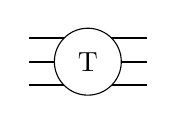
\begin{tikzpicture}[baseline=0cm,scale=\scl]
  \var
  \draw[thick] ({-\xt},{\yt}) -- (\xt,{\yt});
  \draw[thick] ({-\xt},0) -- (\xt,0);
  \draw[thick] ({-\xt},{-\yt}) -- (\xt,{-\yt});
  % \fill[black] (0,{-\yt}) circle [radius=0.4];
  \node[circle,draw,inner sep=0pt,minimum size=\Rad, fill=white] () at (0,0) {T};
\end{tikzpicture}
}

\newcommand{\stattThree}{
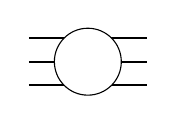
\begin{tikzpicture}[baseline=0cm,scale=\scl]
  \var
  \draw[thick] ({-\xt},{\yt}) -- (\xt,{\yt});
  \draw[thick] ({-\xt},0) -- (\xt,0);
  \draw[thick] ({-\xt},{-\yt}) -- (\xt,{-\yt});
  % \fill[black] (0,{-\yt}) circle [radius=0.4];
  \node[circle,draw,inner sep=0pt,minimum size=\Rad, fill=white] () at (0,0) {};
\end{tikzpicture}
}

\newcommand{\stattThreeCC}{
\begin{tikzpicture}[baseline=0cm,scale=\scl]
  \var
  \draw[thick] ({-\xt},{\yt}) -- (\xt,{\yt});
  \draw[thick] ({-\xt},0) -- (\xt,0);
  \draw[thick] ({-\xt},{-\yt}) -- (\xt,{-\yt});
  % \fill[black] (0,{-\yt}) circle [radius=0.4];
  \node[circle,draw,inner sep=0pt,minimum size=\Rad, fill=white] () at (0,0) {};
  \node[circle,draw,inner sep=0pt,minimum size=\Rad, fill=white,pattern=north east lines] () at (0,0) {};
\end{tikzpicture}
}

%%%%%%%%%%%%%%%%%%%%%%%%%%%%%%%%%%%%%%%%%%%%%%%%%%%%%%%%%%%%%%%%%%%%%%%%%%%%%%%%%%%
%%%%%%%%%%%%%%%%%%%%%%%%%%%%%%%%%%%%%%%%%%%%%%%%%%%%%%%%%%%%%%%%%%%%%%%%%%%%%%%%%%%
%%%%%%%%%%%%%%%%%%%%%%%%%%%%%%%%%%%%%%%%%%%%%%%%%%%%%%%%%%%%%%%%%%%%%%%%%%%%%%%%%%%
%%%%%%%%%%%%%%%%%%%%%%%%%%%%%%%%%%%%%%%%%%%%%%%%%%%%%%%%%%%%%%%%%%%%%%%%%%%%%%%%%%%
%%%%%%%%%%%%%%%%%%%%%%%%%%%%%%%%%%%%%%%%%%%%%%%%%%%%%%%%%%%%%%%%%%%%%%%%%%%%%%%%%%%

\newcommand{\prodUp}[1]{
\begin{tikzpicture}[baseline=0cm,scale=\scl]
  \var
  \draw[thick,decorate, decoration={snake,amplitude=.4mm,segment length=2mm,post length=0mm}] ({-\xt},0.0) -- ({-\xm},0.0);
%
  \draw[thick] ({\xm},{\yt+\dyt}) -- node[yshift=0.1cm] {\color{black}$#1$} (\xt,{\yt+\dyt});
  \draw[thick] ({\xm},{\yt-\dyt}) -- (\xt,{\yt-\dyt});
  \draw[thick] ({\xm},{-\yt})  -- (\xt, {-\yt});
  % \fill[black] (0,{-\yt}) circle [radius=0.4];
  \node[circle,draw,inner sep=0pt,minimum size=\Rad, fill=white] () at (0,0) {};
  \node[circle,draw,inner sep=0pt,minimum size=\Rad, fill=white,pattern=crosshatch dots] () at (0,0) {};
\end{tikzpicture}
}

%%%%%%%%%%%%%%%%%%%%%%%%%%%%%%%%%%%%%%%%%%%%%%%%%%%%%%%%%%%%%%%%%%%%%%%%%%%%%%%%%%%
%%%%%%%%%%%%%%%%%%%%%%%%%%%%%%%%%%%%%%%%%%%%%%%%%%%%%%%%%%%%%%%%%%%%%%%%%%%%%%%%%%%
%%%%%%%%%%%%%%%%%%%%%%%%%%%%%%%%%%%%%%%%%%%%%%%%%%%%%%%%%%%%%%%%%%%%%%%%%%%%%%%%%%%
%%%%%%%%%%%%%%%%%%%%%%%%%%%%%%%%%%%%%%%%%%%%%%%%%%%%%%%%%%%%%%%%%%%%%%%%%%%%%%%%%%%
%%%%%%%%%%%%%%%%%%%%%%%%%%%%%%%%%%%%%%%%%%%%%%%%%%%%%%%%%%%%%%%%%%%%%%%%%%%%%%%%%%%

\newcommand{\KUp}[1]{
\begin{tikzpicture}[baseline=0cm,scale=\scl]
  \var
%
  \draw[thick] ({\xm},{\yt+\dyt}) -- node[yshift=0.1cm] {\color{black}$#1$} (\xt,{\yt+\dyt});
  \draw[thick] ({\xm},{\yt-\dyt}) -- (\xt,{\yt-\dyt});
  \draw[thick] ({\xm},{-\yt})  -- (\xt, {-\yt});
  % \fill[black] (0,{-\yt}) circle [radius=0.4];
  \draw[fill=white] (\xm,0) ellipse ({1.4*\xm} and {1.6*\Rad});
  \node[] () at ({\xm},0) {K};
\end{tikzpicture}
}

\newcommand{\KDn}[1]{
\begin{tikzpicture}[baseline=0cm,scale=\scl]
  \var
%
  \draw[thick] ({\xm},{\yt})  -- node[yshift=0.1cm] {\color{black}$#1$} (\xt, {\yt});
  \draw[thick] ({\xm},{-\yt+\dyt}) -- (\xt,{-\yt+\dyt});
  \draw[thick] ({\xm},{-\yt-\dyt}) -- (\xt,{-\yt-\dyt});
  % \fill[black] (0,{-\yt}) circle [radius=0.4];
  \draw[fill=white] (\xm,0) ellipse ({1.4*\xm} and {1.6*\Rad});
  \node[] () at ({\xm},0) {K};
\end{tikzpicture}
}

%%%%%%%%%%%%%%%%%%%%%%%%%%%%%%%%%%%%%%%%%%%%%%%%%%%%%%%%%%%%%%%%%%%%%%%%%%%%%%%%%%%
%%%%%%%%%%%%%%%%%%%%%%%%%%%%%%%%%%%%%%%%%%%%%%%%%%%%%%%%%%%%%%%%%%%%%%%%%%%%%%%%%%%
%%%%%%%%%%%%%%%%%%%%%%%%%%%%%%%%%%%%%%%%%%%%%%%%%%%%%%%%%%%%%%%%%%%%%%%%%%%%%%%%%%%
%%%%%%%%%%%%%%%%%%%%%%%%%%%%%%%%%%%%%%%%%%%%%%%%%%%%%%%%%%%%%%%%%%%%%%%%%%%%%%%%%%%
%%%%%%%%%%%%%%%%%%%%%%%%%%%%%%%%%%%%%%%%%%%%%%%%%%%%%%%%%%%%%%%%%%%%%%%%%%%%%%%%%%%

\newcommand{\conUpUp}[2]{\ensuremath{
    \begin{tikzpicture}[baseline=0cm,scale=\scl]
      \var
      \draw[thick] ({-\xt},{\yt+\dyt}) -- node[yshift=0.1cm] {\color{black}$#1$} ({-\xm},{\yt+\dyt});
      \draw[thick] ({-\xt},{\yt-\dyt}) -- ({-\xm},{\yt-\dyt});
      \draw[thick] ({-\xt},{-\yt})  -- ({-\xm}, {-\yt});
%
      \draw[thick] ({\xm},{\yt+\dyt}) -- node[yshift=0.1cm] {\color{black}$#2$} (\xt,{\yt+\dyt});
      \draw[thick] ({\xm},{\yt-\dyt}) -- (\xt,{\yt-\dyt});
      \draw[thick] ({\xm},{-\yt})  -- (\xt, {-\yt});
  % \fill[black] (0,{-\yt}) circle [radius=0.4];
      \node[circle,draw,inner sep=0pt,minimum size=\Rad, fill=white] () at (0,0) {};
      \node[circle,draw,inner sep=0pt,minimum size=\Rad, fill=white,pattern=north east lines] () at (0,0) {};
    \end{tikzpicture}}}

    \newcommand{\conRhoRho}{\ensuremath{
        \begin{tikzpicture}[baseline=0cm,scale=\scl]
          \var
          \draw[thick] ({-\xt},{\yt+\dyt}) -- node[yshift=0.1cm] {\color{black}$\xi$} ({-\xm},{\yt+\dyt});
          \node[] at ({-1.3*\xt},{\yt-\dyt/2}) {$\sigma\{$};
          \node[] at ({-1.8*\xt},{\yt/2-\dyt}) {$\scalebox{1}[2.2]{\{}$};
          \node[] at ({-2.3*\xt},{\yt/2-\dyt/2}) {$s$};
          \draw[thick] ({-\xt},{\yt-\dyt}) -- ({-\xm},{\yt-\dyt});
          \draw[thick] ({-\xt},{-\yt})  -- ({-\xm}, {-\yt});
    %
          \draw[thick] ({\xm},{\yt+\dyt}) -- node[yshift=0.1cm] {\color{black}$\xi$} (\xt,{\yt+\dyt});
          \node[] at ({1.3*\xt},{\yt-\dyt/2}) {$\}\sigma'$};
          \draw[thick] ({\xm},{\yt-\dyt}) -- (\xt,{\yt-\dyt});
          \draw[thick] ({\xm},{-\yt})  -- (\xt, {-\yt});
      % \fill[black] (0,{-\yt}) circle [radius=0.4];
          \node[circle,draw,inner sep=0pt,minimum size=\Rad, fill=white] () at (0,0) {};
          \node[circle,draw,inner sep=0pt,minimum size=\Rad, fill=white,pattern=north east lines] () at (0,0) {};
        \end{tikzpicture}}}


%% Down Up
\newcommand{\conDnUp}[2]{\ensuremath{
        \begin{tikzpicture}[baseline=0cm,scale=\scl]
          \var
          \draw[thick] ({-\xt},\yt) -- node[yshift=0.1cm] {\color{black}$#1$} ({-\xm},\yt);
          \draw[thick] ({-\xt},{-\yt+\dyt}) -- ({-\xm},{-\yt+\dyt});
          \draw[thick] ({-\xt},{-\yt-\dyt})  -- ({-\xm}, {-\yt-\dyt});
%
          \draw[thick] ({\xm},{\yt+\dyt}) -- node[yshift=0.1cm] {\color{black}$#2$} (\xt,{\yt+\dyt});
          \draw[thick] ({\xm},{\yt-\dyt}) -- (\xt,{\yt-\dyt});
          \draw[thick] (0,{-\yt})  -- (\xt, {-\yt});
%
          \node[circle,draw,inner sep=0pt,minimum size=\Rad, fill=white] () at (0,0) {};
          \node[circle,draw,inner sep=0pt,minimum size=\Rad, fill=white,pattern=north east lines] () at (0,0) {};
        \end{tikzpicture}}}

%% Up Down
\newcommand{\conUpDn}[2]{\ensuremath{
        \begin{tikzpicture}[baseline=0cm,scale=\scl]
          \var
          \draw[thick] ({-\xt},{\yt+\dyt}) -- node[yshift=0.1cm] {\color{black}$#1$} ({-\xm},{\yt+\dyt});
          \draw[thick] ({-\xt},{\yt-\dyt}) -- ({-\xm},{\yt-\dyt});
          \draw[thick] ({-\xt},{-\yt})  -- ({-\xm}, {-\yt});
%
          \draw[thick] ({\xm},\yt) -- node[yshift=0.1cm] {\color{black}$#2$} (\xt,\yt);
          \draw[thick] ({\xm},{-\yt+\dyt}) -- (\xt,{-\yt+\dyt});
          \draw[thick] ({\xm},{-\yt-\dyt})  -- (\xt, {-\yt-\dyt});
  % \fill[black] (0,{-\yt}) circle [radius=0.4];
          \node[circle,draw,inner sep=0pt,minimum size=\Rad, fill=white] () at (0,0) {};
          \node[circle,draw,inner sep=0pt,minimum size=\Rad, fill=white,pattern=north east lines] () at (0,0) {};
        \end{tikzpicture}}}

%%%%%%%%%%%%%%%%%%%%%%%%%%%%%%%%%%%%%%%%%%%%%%%%%%%%%%%%%%%%%%%%%%%%%%%%%%%%%%%%%%%
%%%%%%%%%%%%%%%%%%%%%%%%%%%%%%%%%%%%%%%%%%%%%%%%%%%%%%%%%%%%%%%%%%%%%%%%%%%%%%%%%%%
%%%%%%%%%%%%%%%%%%%%%%%%%%%%%%%%%%%%%%%%%%%%%%%%%%%%%%%%%%%%%%%%%%%%%%%%%%%%%%%%%%%
%%%%%%%%%%%%%%%%%%%%%%%%%%%%%%%%%%%%%%%%%%%%%%%%%%%%%%%%%%%%%%%%%%%%%%%%%%%%%%%%%%%
%%%%%%%%%%%%%%%%%%%%%%%%%%%%%%%%%%%%%%%%%%%%%%%%%%%%%%%%%%%%%%%%%%%%%%%%%%%%%%%%%%%

\newcommand{\RUpUp}[2]{\ensuremath{
    \begin{tikzpicture}[baseline=0cm,scale=\scl]
      \var
      \draw[thick] ({-\xt},{\yt+\dyt}) -- node[yshift=0.1cm] {\color{black}$#1$} ({-\xm},{\yt+\dyt});
      \draw[thick] ({-\xt},{\yt-\dyt}) -- ({-\xm},{\yt-\dyt});
      \draw[thick] ({-\xt},{-\yt})  -- ({-\xm}, {-\yt});
%
      \draw[thick] ({\xm},{\yt+\dyt}) -- node[yshift=0.1cm] {\color{black}$#2$} (\xt,{\yt+\dyt});
      \draw[thick] ({\xm},{\yt-\dyt}) -- (\xt,{\yt-\dyt});
      \draw[thick] ({\xm},{-\yt})  -- (\xt, {-\yt});
  % \fill[black] (0,{-\yt}) circle [radius=0.4];
      \node[circle,draw,inner sep=0pt,minimum size=\Rad, fill=white] () at (0,0) {R};
%      \node[circle,draw,inner sep=0pt,minimum size=\Rad, fill=white,pattern=north east lines] () at (0,0) {};
    \end{tikzpicture}}}

\newcommand{\LUpUp}[2]{\ensuremath{
    \begin{tikzpicture}[baseline=0cm,scale=\scl]
      \var
      \draw[thick] ({-\xt},{\yt+\dyt}) -- node[yshift=0.1cm] {\color{black}$#1$} ({-\xm},{\yt+\dyt});
      \draw[thick] ({-\xt},{\yt-\dyt}) -- ({-\xm},{\yt-\dyt});
      \draw[thick] ({-\xt},{-\yt})  -- ({-\xm}, {-\yt});
%
      \draw[thick] ({\xm},{\yt+\dyt}) -- node[yshift=0.1cm] {\color{black}$#2$} (\xt,{\yt+\dyt});
      \draw[thick] ({\xm},{\yt-\dyt}) -- (\xt,{\yt-\dyt});
      \draw[thick] ({\xm},{-\yt})  -- (\xt, {-\yt});
  % \fill[black] (0,{-\yt}) circle [radius=0.4];
      \node[circle,draw,inner sep=0pt,minimum size=\Rad, fill=white] () at (0,0) {L};
%      \node[circle,draw,inner sep=0pt,minimum size=\Rad, fill=white,pattern=north east lines] () at (0,0) {};
    \end{tikzpicture}}}

\newcommand{\RUpDn}[2]{\ensuremath{
        \begin{tikzpicture}[baseline=0cm,scale=\scl]
          \var
          \draw[thick] ({-\xt},{\yt+\dyt}) -- node[yshift=0.1cm] {\color{black}$#1$} ({-\xm},{\yt+\dyt});
          \draw[thick] ({-\xt},{\yt-\dyt}) -- ({-\xm},{\yt-\dyt});
          \draw[thick] ({-\xt},{-\yt})  -- ({-\xm}, {-\yt});
%
          \draw[thick] ({\xm},\yt) -- node[yshift=0.1cm] {\color{black}$#2$} (\xt,\yt);
          \draw[thick] ({\xm},{-\yt+\dyt}) -- (\xt,{-\yt+\dyt});
          \draw[thick] ({\xm},{-\yt-\dyt})  -- (\xt, {-\yt-\dyt});
  % \fill[black] (0,{-\yt}) circle [radius=0.4];
          \node[circle,draw,inner sep=0pt,minimum size=\Rad, fill=white] () at (0,0) {R};
  % \node[circle,draw,inner sep=0pt,minimum size=\Rad, fill=white,pattern=north east lines] () at (0,0) {};
        \end{tikzpicture}}}
\newcommand{\LUpDn}[2]{\ensuremath{
            \begin{tikzpicture}[baseline=0cm,scale=\scl]
              \var
              \draw[thick] ({-\xt},{\yt+\dyt}) -- node[yshift=0.1cm] {\color{black}$#1$} ({-\xm},{\yt+\dyt});
              \draw[thick] ({-\xt},{\yt-\dyt}) -- ({-\xm},{\yt-\dyt});
              \draw[thick] ({-\xt},{-\yt})  -- ({-\xm}, {-\yt});
%
              \draw[thick] ({\xm},\yt) -- node[yshift=0.1cm] {\color{black}$#2$} (\xt,\yt);
              \draw[thick] ({\xm},{-\yt+\dyt}) -- (\xt,{-\yt+\dyt});
              \draw[thick] ({\xm},{-\yt-\dyt})  -- (\xt, {-\yt-\dyt});
      % \fill[black] (0,{-\yt}) circle [radius=0.4];
              \node[circle,draw,inner sep=0pt,minimum size=\Rad, fill=white] () at (0,0) {L};
      % \node[circle,draw,inner sep=0pt,minimum size=\Rad, fill=white,pattern=north east lines] () at (0,0) {};
            \end{tikzpicture}}}

%%%%%%%%%%%%%%%%%%%%%%%%%%%%%%%%%%%%%%%%%%%%%%%%%%%%%%%%%%%%%%%%%%%%%%%%%%%%%%%%%%%
%%%%%%%%%%%%%%%%%%%%%%%%%%%%%%%%%%%%%%%%%%%%%%%%%%%%%%%%%%%%%%%%%%%%%%%%%%%%%%%%%%%
%%%%%%%%%%%%%%%%%%%%%%%%%%%%%%%%%%%%%%%%%%%%%%%%%%%%%%%%%%%%%%%%%%%%%%%%%%%%%%%%%%%
%%%%%%%%%%%%%%%%%%%%%%%%%%%%%%%%%%%%%%%%%%%%%%%%%%%%%%%%%%%%%%%%%%%%%%%%%%%%%%%%%%%
%%%%%%%%%%%%%%%%%%%%%%%%%%%%%%%%%%%%%%%%%%%%%%%%%%%%%%%%%%%%%%%%%%%%%%%%%%%%%%%%%%%

\newcommand{\disUpUp}[2]{\ensuremath{
    \begin{tikzpicture}[baseline=0cm,scale=\scl]
      \var
      \draw[thick] ({-\xt},{\yt+\dyt}) -- node[yshift=0.1cm] {\color{black}$#1$} ({-\xm},{\yt+\dyt});
      \draw[thick] ({-\xt},{\yt-\dyt}) -- ({-\xm},{\yt-\dyt});
      \draw[thick] ({-\xt},{-\yt})  -- (0, {-\yt});
%
      \draw[thick] ({\xm},{\yt+\dyt}) -- node[yshift=0.1cm] {\color{black}$#2$} (\xt,{\yt+\dyt});
      \draw[thick] ({\xm},{\yt-\dyt}) -- (\xt,{\yt-\dyt});
      \draw[thick] (0,{-\yt})  -- (\xt, {-\yt});
%
  % \fill[black] (0,{-\yt}) circle [radius=0.4];
      \node[circle,draw,inner sep=0pt,minimum size=\rad, fill=white] () at (0,1) {};
    \end{tikzpicture}}}

\newcommand{\disDnDn}[2]{\ensuremath{
        \begin{tikzpicture}[baseline=0cm,scale=\scl]
          \var
          \draw[thick] ({-\xt},\yt) -- node[yshift=0.1cm] {\color{black}$#1$} ((0,\yt);
          \draw[thick] ({-\xt},{-\yt+\dyt}) -- ({-\xm},{-\yt+\dyt});
          \draw[thick] ({-\xt},{-\yt-\dyt})  -- {-\xm}, {-\yt-\dyt});
%
          \draw[thick] (0,\yt) -- node[yshift=0.1cm] {\color{black}$#2$} (\xt,\yt);
          \draw[thick] ({\xm},{-\yt+\dyt}) -- (\xt,{-\yt+\dyt});
          \draw[thick] ({\xm},{-\yt-\dyt})  -- (\xt, {-\yt-\dyt});
%
  % \fill[black] (0,{-\yt}) circle [radius=0.4];
          \node[circle,draw,inner sep=0pt,minimum size=\rad, fill=white] () at (0,{-\yt}) {};
        \end{tikzpicture}}}

%%%%%%%%%%%%%%%%%%%%%%%%%%%%%%%%%%%%%%%%%%%%%%%%%%%%%%%%%%%%%%%%%%%%%%%%%%%%%%%%%%%
%%%%%%%%%%%%%%%%%%%%%%%%%%%%%%%%%%%%%%%%%%%%%%%%%%%%%%%%%%%%%%%%%%%%%%%%%%%%%%%%%%%
%%%%%%%%%%%%%%%%%%%%%%%%%%%%%%%%%%%%%%%%%%%%%%%%%%%%%%%%%%%%%%%%%%%%%%%%%%%%%%%%%%%
%%%%%%%%%%%%%%%%%%%%%%%%%%%%%%%%%%%%%%%%%%%%%%%%%%%%%%%%%%%%%%%%%%%%%%%%%%%%%%%%%%%
%%%%%%%%%%%%%%%%%%%%%%%%%%%%%%%%%%%%%%%%%%%%%%%%%%%%%%%%%%%%%%%%%%%%%%%%%%%%%%%%%%%

\newcommand{\recopDnUp}{\ensuremath{
    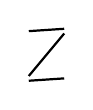
\begin{tikzpicture}[baseline=0cm,scale=\scl]
      \var
      \draw[thick] ({-\xt/2},\yt) -- ({\xm/2},{\yt+\dyt});
      \draw[thick] ({-\xt/2},{-\yt+\dyt}) -- ({\xm/2},{\yt-\dyt});
      \draw[thick] ({-\xt/2},{-\yt-\dyt})  -- ({\xm/2}, -\yt);
    \end{tikzpicture}}}

\newcommand{\recopUpDn}{\ensuremath{
    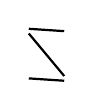
\begin{tikzpicture}[baseline=0cm,scale=\scl]
      \var
      \draw[thick] ({-\xt/2},{\yt+\dyt}) -- ({\xm/2},\yt);
      \draw[thick] ({-\xt/2},{\yt-\dyt}) -- ({\xm/2},{-\yt+\dyt});
      \draw[thick] ({-\xt/2},{-\yt})  -- ({\xm/2}, {-\yt-\dyt});
    \end{tikzpicture}}}

%%%%%%%%%%%%%%%%%%%%%%%%%%%%%%%%%%%%%%%%%%%%%%%%%%%%%%%%%%%%%%%%%%%%%%%%%%%%%%%%%%%
%%%%%%%%%%%%%%%%%%%%%%%%%%%%%%%%%%%%%%%%%%%%%%%%%%%%%%%%%%%%%%%%%%%%%%%%%%%%%%%%%%%
%%%%%%%%%%%%%%%%%%%%%%%%%%%%%%%%%%%%%%%%%%%%%%%%%%%%%%%%%%%%%%%%%%%%%%%%%%%%%%%%%%%
%%%%%%%%%%%%%%%%%%%%%%%%%%%%%%%%%%%%%%%%%%%%%%%%%%%%%%%%%%%%%%%%%%%%%%%%%%%%%%%%%%%
%%%%%%%%%%%%%%%%%%%%%%%%%%%%%%%%%%%%%%%%%%%%%%%%%%%%%%%%%%%%%%%%%%%%%%%%%%%%%%%%%%%

\newcommand{\opeDnUp}[2]{\ensuremath{
    \begin{tikzpicture}[baseline=0cm,scale=\scl]
      \var
      \draw[thick] ({-\xt},\yt) -- node[yshift=0.1cm] {\color{black}$#1$} ({\xm},{\yt+\dyt}) -- node[yshift=0.1cm] {\color{black}$#2$} ({\xt},{\yt+\dyt});
      \draw[thick] ({-\xt},{-\yt+\dyt}) -- ({-\xm},{-\yt+\dyt}) -- ({\xm},{\yt-\dyt}) -- (\xt,{\yt-\dyt});
      \draw[thick] ({-\xt},{-\yt-\dyt}) -- ({-\xm},{-\yt-\dyt})-- (\xt, -\yt);
%
      \node[circle,draw,inner sep=0pt,minimum size=\rad, fill=white] () at ({-\xm},{-\yt}) {};
      \node[circle,draw,inner sep=0pt,minimum size=\rad, fill=white] () at ({\xm},{\yt}) {};
    \end{tikzpicture}}}

\newcommand{\opeUpDn}[2]{\ensuremath{
    \begin{tikzpicture}[baseline=0cm,scale=\scl]
      \var
      \draw[thick] ({-\xt},{\yt+\dyt}) -- node[yshift=0.1cm] {\color{black}$#1$} ({-\xm},{\yt+\dyt}) -- node[yshift=0.1cm] {\color{black}$#2$} (\xt, \yt);
      \draw[thick] ({-\xt},{\yt-\dyt}) -- ({-\xm},{\yt-\dyt}) -- ({\xm},{-\yt+\dyt}) -- (\xt,{-\yt+\dyt});
      \draw[thick] ({-\xt},-\yt) -- ({\xm},{-\yt-\dyt}) -- ({\xt},{-\yt-\dyt});
%
      \node[circle,draw,inner sep=0pt,minimum size=\rad, fill=white] () at ({-\xm},{\yt}) {};
      \node[circle,draw,inner sep=0pt,minimum size=\rad, fill=white] () at ({\xm},{-\yt}) {};
    \end{tikzpicture}}}


%%%%%%%%%%%%%%%%%%%%%%%%%%%%%%%%%%%%%%%%%%%%%%%%%%%%%%%%%%%%%%%%%%%%%%%%%%%%%%%%%%%
%%%%%%%%%%%%%%%%%%%%%%%%%%%%%%%%%%%%%%%%%%%%%%%%%%%%%%%%%%%%%%%%%%%%%%%%%%%%%%%%%%%
%%%%%%%%%%%%%%%%%%%%%%%%%%%%%%%%%%%%%%%%%%%%%%%%%%%%%%%%%%%%%%%%%%%%%%%%%%%%%%%%%%%
%%%%%%%%%%%%%%%%%%%%%%%%%%%%%%%%%%%%%%%%%%%%%%%%%%%%%%%%%%%%%%%%%%%%%%%%%%%%%%%%%%%
%%%%%%%%%%%%%%%%%%%%%%%%%%%%%%%%%%%%%%%%%%%%%%%%%%%%%%%%%%%%%%%%%%%%%%%%%%%%%%%%%%%

\newcommand{\uniIso}[3]{\ensuremath{
    \begin{tikzpicture}[baseline=0cm,scale=\scl]
      \var
      \draw[thick] ({-\xt},{\yt+\dyt}) -- ({-\xm},{\yt+\dyt});
      \draw[thick] ({-\xt},{\yt-\dyt}) -- ({-\xm},{\yt-\dyt});
      \draw[thick] ({-\xt},{-\yt})  -- ({-\xm}, {-\yt});
%
      \draw[thick] ({\xm},{\yt+\dyt}) -- (\xt,{\yt+\dyt});
      \draw[thick] ({\xm},{\yt-\dyt}) -- (\xt,{\yt-\dyt});
      \draw[thick] ({\xm},{-\yt})  -- (\xt, {-\yt});
  % \fill[black] (0,{-\yt}) circle [radius=0.4];
      \node[circle,draw,inner sep=0pt,minimum size=\Rad, fill=white] () at (0,0) {};
      \node[] at (0,{-\Rad*0.5}) {{$#2$}};
      \node[] at ({-0.8*\Rad},{\Rad*0.9}) {\tiny{$#1$}};
      \node[] at ({0.8*\Rad},{\Rad*0.9}) {\tiny{$#3$}};
      \draw[] (0,{1.6*\Rad}) to[out=270,in=180] ({1.6*\Rad},0);
      \draw[] (0,{1.6*\Rad}) to[out=270,in=0] ({-1.6*\Rad},0);
    \end{tikzpicture}}}

%%%%%%%%%%%%%%%%%%%%%%%%%%%%%%%%%%%%%%%%%%%%%%%%%%%%%%%%%%%%%%%%%%%%%%%%%%%%%%%%%%%
%%%%%%%%%%%%%%%%%%%%%%%%%%%%%%%%%%%%%%%%%%%%%%%%%%%%%%%%%%%%%%%%%%%%%%%%%%%%%%%%%%%
%%%%%%%%%%%%%%%%%%%%%%%%%%%%%%%%%%%%%%%%%%%%%%%%%%%%%%%%%%%%%%%%%%%%%%%%%%%%%%%%%%%
%%%%%%%%%%%%%%%%%%%%%%%%%%%%%%%%%%%%%%%%%%%%%%%%%%%%%%%%%%%%%%%%%%%%%%%%%%%%%%%%%%%
%%%%%%%%%%%%%%%%%%%%%%%%%%%%%%%%%%%%%%%%%%%%%%%%%%%%%%%%%%%%%%%%%%%%%%%%%%%%%%%%%%%


\newcommand{\Ksum}{
    \ensuremath{
    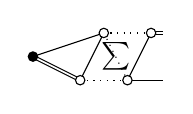
\begin{tikzpicture}[baseline=0cm,scale=\scl]
      \var
%
      \draw[]  (0,0) -- (3.0,{ \yt});
      \draw[double] (0,0) -- (2.0,{-\yt});
      \draw[fill=black] (0,0) ellipse (0.2);
%
      \draw[] (2.0,{-\yt}) -- (3.0,{ \yt});
      \draw[dotted] (3.0,{ \yt}) -- node[] {\tiny $\sum$} (4.0,{-\yt});
      \draw[] (4.0,{-\yt}) -- (5.0,{+\yt});
%
      \draw[dotted] (2.0,{-\yt}) -- (4.0,{-\yt});
      \draw[dotted] (3.0,{ \yt}) -- (5.0,{ \yt});
%
      \draw[double] (5.0,{ \yt}) -- (5.5,{ \yt});
      \draw[] (4.0,{-\yt}) -- (5.5,{-\yt});
      \draw[fill=white] (2.0,-\yt) ellipse (0.2);
      \draw[fill=white] (3.0,\yt) ellipse (0.2);
      \draw[fill=white] (4.0,-\yt) ellipse (0.2);
      \draw[fill=white] (5.0,+\yt) ellipse (0.2);
    \end{tikzpicture}
    }}

\newcommand{\Ladder}{
\ensuremath{
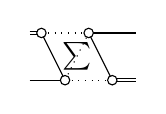
\begin{tikzpicture}[baseline=0cm,scale=\scl]
  \var
  \draw[double] (4.5,{\yt})  -- (5.0,{\yt});
  \draw[]       (4.5,{-\yt}) -- (6.0,{-\yt});
  \draw[] (5.0,{ \yt}) -- (6.0,{-\yt});
  \draw[dotted] (5.0,{ \yt}) -- (7.0,{ \yt});
  \draw[dotted] (6.0,{-\yt}) -- node[] {\tiny $\sum$} (7.0,{\yt});
  \draw[dotted] (6.0,{-\yt}) -- (8.0,{-\yt});
  \draw[] (7.0,{ \yt}) -- (8.0,{-\yt});
  \draw[] (7.0,{ \yt}) -- (9.0,{ \yt});
  \draw[double] (8.0,{-\yt}) -- (9.0,{-\yt});
%
  \draw[fill=white] (5.0,\yt) ellipse (0.2);
  \draw[fill=white] (6.0,-\yt) ellipse (0.2);
  \draw[fill=white] (7.0,\yt) ellipse (0.2);
  \draw[fill=white] (8.0,-\yt) ellipse (0.2);
\end{tikzpicture}
}
}

\newcommand{\K}{
\ensuremath{
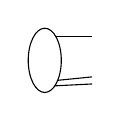
\begin{tikzpicture}[baseline=0cm,scale=\scl]
  \var
%
  \draw[]  (0,{ \yt}) -- (2.0,{ \yt});
  \draw[] (0,{-\yt+\dyt}) -- (2.0,{-\yt+3*\dyt});
  \draw[] (0,{-\yt-\dyt}) -- (2.0,{-\yt});
  % \draw[double] (0,{-\yt}) -- (2.0,{-\yt});
  \draw[fill=white] (0,0) ellipse ({1.4*\xm} and {1.6*\Rad});
  % \node[] () at ({\xm},0) {};
\end{tikzpicture}
}
}

    %%%%%%%%%%%%%%%%%%%%%%%%%%%%%%%%%%%%%%%%%%%%%%%%%%%%%%%%%%%%%%%%%%%%%%%%%%%%%%%%%%%
    %%%%%%%%%%%%%%%%%%%%%%%%%%%%%%%%%%%%%%%%%%%%%%%%%%%%%%%%%%%%%%%%%%%%%%%%%%%%%%%%%%%
    %%%%%%%%%%%%%%%%%%%%%%%%%%%%%%%%%%%%%%%%%%%%%%%%%%%%%%%%%%%%%%%%%%%%%%%%%%%%%%%%%%%
    %%%%%%%%%%%%%%%%%%%%%%%%%%%%%%%%%%%%%%%%%%%%%%%%%%%%%%%%%%%%%%%%%%%%%%%%%%%%%%%%%%%
    %%%%%%%%%%%%%%%%%%%%%%%%%%%%%%%%%%%%%%%%%%%%%%%%%%%%%%%%%%%%%%%%%%%%%%%%%%%%%%%%%%%

\newcommand{\res}{
    \ensuremath{
    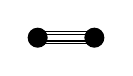
\begin{tikzpicture}[baseline=0cm,scale=\scl]
      \var%
      \draw[double]  (-1.2,0.2) -- (1.2,0.2);
      \draw[double]  (-1.2,-0.2) -- (1.2,-0.2);
      \draw[fill=black] (1.2,0) ellipse (0.4);
      \draw[fill=black] (-1.2,0) ellipse (0.4);
    \end{tikzpicture}
    }}
